%%%%%%%%%%%%%%%%%%%%%%%%%%%%%%%%%%%%%%%%%
% Class Notes Template
% LaTeX Template
% By: Ryan Grove
%%%%%%%%%%%%%%%%%%%%%%%%%%%%%%%%%%%%%%%%%

%----------------------------------------------------------------------------------------
%	PACKAGES AND OTHER DOCUMENT CONFIGURATIONS
%----------------------------------------------------------------------------------------

\documentclass[paper=a4, fontsize=11pt]{scrartcl} % A4 paper and 11pt font size

\usepackage[T1]{fontenc} % Use 8-bit encoding that has 256 glyphs
\usepackage{fourier} % Use the Adobe Utopia font for the document - comment this line to return to the LaTeX default
\usepackage[english]{babel} % English language/hyphenation
\usepackage{amsmath,amsfonts,amsthm} % Math packages

\usepackage{lipsum} % Used for inserting dummy 'Lorem ipsum' text into the template

\usepackage{sectsty} % Allows customizing section commands
\allsectionsfont{\centering \normalfont\scshape} % Make all sections centered, the default font and small caps

\usepackage{fancyhdr} % Custom headers and footers
\pagestyle{fancyplain} % Makes all pages in the document conform to the custom headers and footers
\fancyhead{} % No page header - if you want one, create it in the same way as the footers below
\fancyfoot[L]{} % Empty left footer
\fancyfoot[C]{} % Empty center footer
%\fancyfoot[R]{\thepage} % Page numbering for right footer
\renewcommand{\headrulewidth}{0pt} % Remove header underlines
\renewcommand{\footrulewidth}{0pt} % Remove footer underlines
\setlength{\headheight}{13.6pt} % Customize the height of the header

\numberwithin{equation}{section} % Number equations within sections (i.e. 1.1, 1.2, 2.1, 2.2 instead of 1, 2, 3, 4)
\numberwithin{figure}{section} % Number figures within sections (i.e. 1.1, 1.2, 2.1, 2.2 instead of 1, 2, 3, 4)
\numberwithin{table}{section} % Number tables within sections (i.e. 1.1, 1.2, 2.1, 2.2 instead of 1, 2, 3, 4)

\setlength\parindent{0pt} % Removes all indentation from paragraphs - comment this line for an assignment with lots of text

\usepackage{lastpage}
\usepackage{fancyhdr}
\cfoot{\thepage\ of \pageref{LastPage}}

\def\v{\hbox{$\mathbf v$}}
\def\w{\hbox{$\mathbf w$}}
\def\u{\hbox{$\mathbf u$}}
\def\x{\hbox{$\textbf{x}$}}
\def\z{\hbox{$\mathbf z$}}
\def\a{\hbox{$\mathbf a$}}
\def\b{\hbox{$\mathbf b$}}
\def\L{\hbox{$\mathcal L$}}
\def\C{\hbox{$\mathbb C$}}
\def\B{\hbox{$\mathcal B$}}
\def\R{\hbox{$\mathbb R$}}
\def\X{\hbox{$\underline X$}}
\def\Q{\hbox{$\mathbb Q$}}
\def\R{\hbox{$\mathbb R$}}
\def\N{\hbox{$\mathbb N$}}
\def\C{\hbox{$\mathbb C$}}
\def\0{\hbox{$\mathbf 0$}}
\def\Y{\hbox{$\underline Y$}}
\def\a{\hbox{$\mathbf a$}}
\def\u{\hbox{$\mathbf u$}}
\def\w{\hbox{$\mathbf w$}}
\def\y{\hbox{$\mathbf y$}}
\def\X{\hbox{$\underline X$}}
\def\dd{\hbox{$\partial $}}
\def\B{\hbox{$\mathcal B$}}
\def\F{\hbox{$\mathcal F$}}
\def\L{\hbox{$\mathcal L$}}
\def\M{\hbox{$\mathcal M$}}
\def\D{\hbox{$\mathscr {D}$}}
\def\RR{\hbox{$\mathscr{R}$}}
\def\I{\hbox{$\mathcal I$}}

\usepackage{amssymb}
%\theoremstyle{plain}
\usepackage[margin = .75in]{geometry}
\newtheorem{claim}{Claim}
\newtheorem{theorem}{Theorem}[section]
\newtheorem{lemma}[theorem]{Lemma}
\newtheorem{proposition}[theorem]{Proposition}
\newtheorem{corollary}[theorem]{Corollary}
\newtheorem{problem}[theorem]{Problem}
%\theoremstyle{definition}
\newtheorem{definition}[theorem]{Definition}
%\theoremstyle{remark}
\newtheorem{remark}[theorem]{Remark}
\newtheorem{remarks}[theorem]{Remarks}
\newtheorem{example}[theorem]{Example}
\newcommand{\ds}{\displaystyle}
\newcommand{\ZZ}{\mathbb{Z}}
\newcommand{\QQ}{\mathbb{Q}}
\newcommand{\e}{\varepsilon}
\newcommand{\bbf}{\textbf}
\newcommand{\p}{\parallel}
\usepackage{color}
\newcommand{\field}[1]{\mathbb{#1}}
\usepackage{amsmath}
\usepackage{amsthm}
\usepackage{amssymb}
\usepackage{mathrsfs}
\usepackage{cancel}
\usepackage{upgreek}
\usepackage{graphicx}
\usepackage{multirow}
\usepackage{setspace}
\usepackage{url}
\usepackage{subfigure}
\usepackage{enumerate}
\usepackage{cases}
\usepackage{mathrsfs}
\usepackage{rotating}

%----------------------------------------------------------------------------------------
%	TITLE SECTION
%----------------------------------------------------------------------------------------

\newcommand{\horrule}[1]{\rule{\linewidth}{#1}} % Create horizontal rule command with 1 argument of height

\title{	
\normalfont \normalsize 
\textsc{Ryan Grove, Clemson University, MATH1080 - 9} \\ [25pt] % Your name, university, class
\horrule{0.5pt} \\[0.4cm] % Thin top horizontal rule
\huge Section 11.2: Series \\ % The assignment title
\horrule{2pt} \\[0.5cm] % Thick bottom horizontal rule
}

\author{Date:} % The due date

\date{\normalsize February 24, 2016} % A custom date

\begin{document}

\maketitle % Print the title

\begin{flushleft}
\begin{tabular}{l l}
Name: \rule{3.2in}{.01cm}  & {}%Table number: \rule{1in}{.01cm}\\
\end{tabular}
\end{flushleft}

%----------------------------------------------------------------------------------------
%	Lecture
%----------------------------------------------------------------------------------------

\section*{\textbf{Lecture:}}
What do we mean when we express a number as an infinite decimal? For instance, what does it mean to write
\[\pi = 3.14159\text{ }26535\text{ }89793\text{ }23846\text{ }26433\text{ }83279\text{ }50288\ldots\]

The convention behind our decimal notation is that any number can be written as an infinite sum. Here it means that
\[\pi = 3 + \ds\frac{1}{10} + \ds\frac{4}{10^2} + \ds\frac{1}{10^3} + \ds\frac{5}{10^4} + \ds\frac{9}{10^5} + \ds\frac{2}{10^6} = \ds\frac{6}{10^7} + \ds\frac{5}{10^8} + \cdots\]

where the three dots $(\cdots)$ indicate that the sum continues forever, and the more terms we add, the closer we get to the actual value of $\pi$.\\
\indent

In general, if we try to add the terms of an infinite sequence $\{a_n\}_{n=1}^\infty$ we get an expression of the form
\[a_1 + a_2 + a_3 + \cdots + a_n + \cdots\]

which is called an \textbf{infinite series} (or just a \underline{\hspace{1in}}) and is denoted, for short, by the symbol
\[\ds\sum_{n=1}^\infty a_n \quad \text{ or } \quad \ds\sum a_n\]
\indent

Does it make sense to talk about the sum of infinitely many terms?\\
\begin{quote}
\flushleft
It would be impossible to find a finite sum for the series
\[1+2+3+4+5+\cdots + n + \cdots\]

because if we start adding the terms we get the cumulative sums $1,3,6,10,15,21,\ldots$and, after the $n$th term, we get $\ds\frac{n(n+1)}{2}$, which becomes very large as $n$ increases (that is, $\ds\sum_{n=1}^\infty n = \infty$).\\
\indent

However, if we start to add the terms of the series
\[\ds\frac{1}{2} + \ds\frac{1}{4} + \ds\frac{1}{8} + \ds\frac{1}{16} + \ds\frac{1}{32} + \ds\frac{1}{64} + \cdots + \ds\frac{1}{2^n} + \cdots\]
\indent

we get $\ds\frac{1}{2},\ds\frac{3}{4},\ds\frac{7}{8},\ds\frac{15}{16},\ds\frac{31}{32},\ds\frac{63}{64},\ldots,\left(1-\ds\frac{1}{2^n}\right),\ldots$. 

\[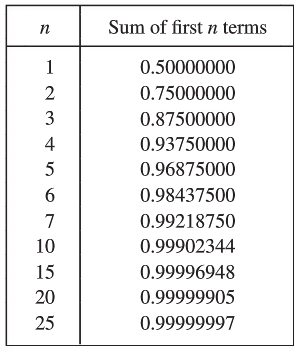
\includegraphics[scale=0.5]{11-2pic1.png}\]

The table shows that as we add more and more terms, these \textit{partial sums} become closer and closer to 1. In fact, by adding sufficiently many terms of the series we can make the partial sums as close as we like to 1. So it seems reasonable to say that the sum of this infinite series is 1 and to write:

\[\ds\sum_{n=1}^\infty \ds\frac{1}{2^n} = \ds\frac{1}{2} + \ds\frac{1}{4} + \ds\frac{1}{8} + \ds\frac{1}{16} + \cdots + \ds\frac{1}{2^n} + \cdots = 1\]
\end{quote}

We use a similar idea to determine whether or not a general series $\ds\sum_{n=1}^\infty a_n$ has a sum. We consider the \underline{\hspace{1in}} \underline{\hspace{0.75in}}
\begin{align*}
s_1 &= a_1\\
s_2 & = a_1 + a_2\\
s_3 & = a_1 + a_2 + a_3\\
s_4 &= a_1 + a_2 + a_3 + a_4
\end{align*}
and in general,
\[S_n = a_1 + a_2 + \cdots + a_n = \ds\sum_{i=1}^n a_i\]

These partial sums form a new sequence $\{S_n\}$, which we call the \textbf{sequence of partial sums}, and which may or may not have a limit. If $\ds\lim_{n\to\infty}S_n = S$ exists (as a finite number), then we call it the sum of the infinite series $\ds\sum_{n=1}^\infty a_n$.\\
\indent

\fbox{
  \parbox{\textwidth}{
  \vspace{5pt} \textbf{\underline{Definition}} Given a series $\ds\sum_{n=1}^\infty a_n = a_1 + a_2 + a_3 + \cdots$, let $S_n$ denote its $n$th partial sum:
  
  \[S_n = \ds\sum_{i=1}^n a_i = a_1 + a_2 + \cdots + a_n\]
  
  \begin{itemize}
  \item If the sequence $\{S_n\}$ is \underline{\hspace{1.25in}} and $\ds\lim_{n\to\infty}S_n = S$ exists as a real number, then the series $\ds\sum_{n=1}^\infty a_n $ is called \underline{\hspace{1.25in}} and we write:
  \[a_1 + a_2 + \cdots + a_n + \cdots = S \quad \text{ or } \quad \ds\sum_{n=1}^\infty a_n = S\]
 where the number $S$ is called the \underline{\hspace{.5in}} of the series.
  \item If the sequence $\{S_n\}$ is \underline{\hspace{1.25in}}, then the series is called \underline{\hspace{1.25in}}.
  \end{itemize}
  
  }}
  \indent\\
  \indent
  
  **Thus, \textbf{the sum of a series is the limit of the sequence of partial sums}.**
  \[\ds\sum_{n=1}^\infty a_n = \ds\lim_{n\to\infty}\ds\sum_{i=1}^n a_i = \ds\lim_{n\to\infty}S_n.\]
  
  \indent
  
  \underline{Example 1}: Suppose we know that the sum of the first $n$ terms of the series $\ds\sum_{n=1}^\infty a_n$ is
  
  \[S_n = a_1 + a_2 + \cdots + a_n = \ds\frac{2n}{3n+5}.\]
  
  Then the sum of the series is the limit of the sequence $\{S_n\}$:
  
  \[\ds\sum_{n=1}^\infty a_n = \hspace{4in}\]
  \indent
  
  It's usually not easy to find such an expression for the sum of the first $n$ terms. However, in Example 2 we look at a famous series for which we \textit{can} find an explicit formula for $S_n$.\\
  \indent
  
  \underline{Example 2}: An important example of an infinite series is the \underline{\hspace{1.25in}} \underline{\hspace{1in}}
  
  \[a + ar + ar^2 + ar^3 + \cdots + ar^{n-1} + \cdots = \ds\sum_{n=1}^\infty ar^{n-1} = \ds\sum_{n=0}^\infty ar^{n} \quad a\neq 0\]
  
  Each term is obtained from the preceding one by multiplying it by the \textbf{common ratio } $\mathbf{r}$.\\
  \indent
  
  \underline{Case 1}: $r=1$\\
  \begin{quote} 
  \flushleft
  Then $S_n = \underbrace{a + a + \cdots + a}_{\text{$n$ copies}} = na \to \pm \infty$. Since $\ds\lim_{n\to\infty}S_n$ doesn't exist, the geometric series diverges in this case.
  \end{quote}
  
  \newpage
  \underline{Case 2}: $r\neq 1$
  \vspace{-25pt}
  \begin{quote}
  \flushleft
  \begin{align*}
  S_n &= a + ar + ar^2 + \cdots + ar^{n-1}\\
  \text{ and } \quad \quad rS_n &= \hspace{20pt} ar + ar^2 + \cdots + ar^{n-1} + ar^n
  \end{align*}
  
  Subtracting these equations gives
  
  \[S_n - rS_n = a - ar^n \quad \implies \quad S_n = \ds\frac{a(1-r^n)}{1-r}\]
  
  If $-1<r<1$, we know that $r^n\to 0$ as $n\to\infty$, so
  \[\ds\lim_{n\to\infty}S_n = \hspace{4in}\]
  \end{quote}
  \indent
  
  Thus when $|r|<1$ the geometric series is convergent and its sum is \underline{\hspace{1in}}.\\
  \indent
  
  If $r\leq -1$ or $r\geq 1$, the sequence $\{r^n\}$ is divergent and so $\ds\lim_{n\to\infty}S_n$ does not exist and therefore, the geometric series diverges.\\
  \indent
  
  \fbox{
  \parbox{\textwidth}{
  \vspace{5pt} \textbf{\underline{Geometric Series}}:
  
  \[\ds\sum_{n=1}^\infty ar^{n-1} = a + ar + ar^2 + \cdots = \ds\sum_{n=0}^\infty ar^n\]
  
  \begin{itemize}
  \item If $|r|<1$, the geometric series is convergent and its sum is $\ds\sum_{n=1}^\infty ar^{n-1} = \ds\frac{a}{1-r} \quad |r|<1$.
  \item If $|r|\geq 1$, the geometric series is divergent.
  \end{itemize}
  
  }}
  \indent\\
  \indent
  
  \underline{Example 3}: Find the sum of the geometric series
  \[5-\ds\frac{10}{3} + \ds\frac{20}{9} - \ds\frac{40}{27} + \cdots\]
  
  \vspace{2in}
  
  \newpage
  \underline{Example 4}: Is the series $\ds\sum_{n=1}^\infty 2^{2n}3^{1-n}$ convergent or divergent?\\
  \indent
  
  \vspace{2.75in}
  
  \underline{Example 5}: Write the number $2.3\overline{17} = 2.3171717\ldots$ as a ratio of integers.\\
  \indent
  
  \vspace{3in}
  
  \underline{Example 6}: Find the sum of the series $\ds\sum_{n=0}^\infty x^n$, where $|x|<1$.\\
  \indent
  
  \textbf{SOLUTION}: Notice that this series starts with $n=0$ and so the first term is $x^0=1$. (With series, we adopt the convention that $x^0=1$ even when $x=0$.) Thus,
  \[\ds\sum_{n=0}^\infty = 1 + x + x^2 + x^3 + x^4 + \cdots\]
  
  This is a geometric series with $a=\underline{\hspace{0.3in}}$ and $r=\underline{\hspace{0.3in}}$. Since $|r|=|x|<1$, it converges and
  
  \[\ds\sum_{n=0}^\infty x_n = \hspace{1in}\]
  \indent\\
  \indent
  
  \underline{Example 7}: Show that the series $\ds\sum_{n=1}^\infty \ds\frac{1}{n(n+1)}$ is convergent, and find its sum.\\
  \indent\\
  \indent
  
  \textbf{SOLUTION}: This is NOT a geometric series, so we go back to the definition of a convergent series and compute the $n$th partial sum:
  
  \[\text{ }\]
  \indent\\
  \indent\\
  \indent
  
  We can simplify this expression if we use the partial fraction decomposition:
  
  \[\text{ }\]
  \indent
  
  Thus,
  \vspace{2.75in}
  
  *\underline{Note}: We call this a \underline{\hspace{1.25in}} \underline{\hspace{0.3in}}. Because of all the cancellation the sum collapses (like a pirate's collapsing telescope) into just two terms.\\
  \indent
  
  And so we then have,
  
  \[\ds\lim_{n\to\infty}S_n = \hspace{3.5in}\]
  \indent\\
  \indent
  
  Therefore, the given series is \underline{\hspace{1.25in}} and \\
  
  \[\text{ }\]
  
  \indent\\
  \indent\\
  \indent
  
  \newpage
  \underline{Example 8}: Show that the \textbf{harmonic series}
  \[\ds\sum_{n=1}^\infty \ds\frac{1}{n} = 1 + \ds\frac{1}{2} + \ds\frac{1}{3} + \ds\frac{1}{4} + \cdots\]
  is divergent.\\
  \indent
  
  \textbf{SOLUTION}: For this particular series it's convenient to consider the partial sums $S_2,S_4,S_8,S_{16},S_{32},\ldots$ and show that they become large.
  
  \[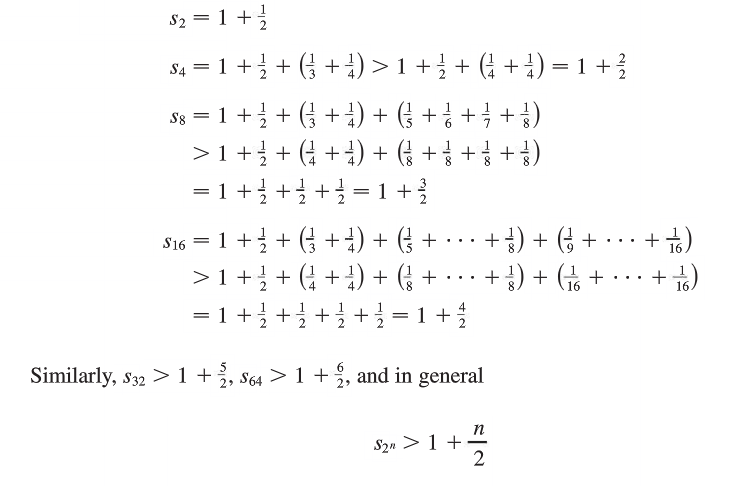
\includegraphics[scale=0.5]{11-2pic2.png}\]
  \indent
  
  This shows that $S_{2^n}\to\infty$ as $n\to\infty$ and so $\{S_n\}$ is divergent. Therefore the harmonic series \underline{\hspace{1in}}.\\
  \indent
  
  \fbox{
  \parbox{\textwidth}{
  \vspace{5pt} \textbf{\underline{Theorem 1}}: \quad If the series $\ds\sum_{n=1}^\infty a_n$ is convergent, then $\ds\lim_{n\to\infty}a_n = 0$.\\
  }}
  \indent\\
  \indent
  
  
  \textbf{PROOF}: 
  \begin{quote}
  \flushleft
  Let $S_n=a_1 + a_2 + \cdots + a_n$. Then $a_n = S_n - S_{n-1}$. Since $\ds\sum_{n=1}^\infty a_n$ is convergent, the sequence $\{S_n\}$ is convergent. Let $\ds\lim_{n\to\infty}S_n=S$. Then also, $\ds\lim_{n\to\infty} S_{n-1}=S$. Therefore,
  
  \[\ds\lim_{n\to\infty} a_n = \hspace{3in}\]
  \end{quote}
  \indent\\
  \indent
  
  \indent
  
  \newpage
  
  \underline{Note 1}: With any \textit{series} $\ds\sum a_n$ we associate two \textit{sequences}:
  \begin{itemize}
  \item $\{S_n\}$: The sequence of its partial sums
  \item $\{a_n\}$: The sequence of its terms
  \end{itemize}
  \begin{quote}
  \flushleft
  \indent If\text{ } $\ds\sum a_n$ is convergent, then the limit of the sequence $\{S_n\}$ is $S$ (the sum of the series) and the limit of the sequence $\{a_n\}=0$.\\
  \end{quote}
  \indent\\
  \indent
  
  \underline{Note 2}: \textbf{The converse of Theorem 1 is not true in general. If $\ds\lim_{n\to\infty}a_n=0$ we cannot \\
  \text{ }\\
  conclude that $\ds\sum a_n$ is convergent}. Consider the harmonic series $\ds\sum \ds\frac{1}{n}$:
  \[a_n = \ds\frac{1}{n} \to 0 \text{ as } n\to\infty, \text{ but as we showed in Example 8}, \ds\sum \ds\frac{1}{n} \text{ is divergent}.\]
  \indent
  
  
  \fbox{
  \parbox{\textwidth}{
  \vspace{5pt} \textbf{\underline{Test for Divergence}}: If $\ds\lim_{n\to\infty} a_n$ does not exist or if $\ds\lim_{n\to\infty} a_n\neq 0$, then the series $\ds\sum_{n=1}^\infty a_n$ is divergent.\\
  }}
  \indent\\
  \indent
  
  The Test for Divergence follows from Theorem 1 because it is a necessary condition that for a series $\ds\sum a_n$ to be convergent $\ds\lim_{n\to\infty} a_n = 0$. Hence, if $\ds\sum_{n\to\infty}a_n\neq 0$, then the series $\ds\sum a_n$ cannot be convergent and must therefore be divergent.\\
  \indent
  
  \underline{Example 9}: Show that the series $\ds\sum_{n=1}^\infty \ds\frac{n^2}{5n^2 + 4}$ diverges.\\
  \indent
  
  \vspace{1.5in}
  
  \underline{Note 3}: 
  \begin{itemize}
  \item If we find that $\ds\lim_{n\to\infty}a_n \neq 0$, we know that $\ds\sum_{a_n}$ is divergent. 
  \item If we find that $\ds\lim_{n\to\infty}a_n = 0$, we know \underline{\hspace{1in}} about the convergence or divergence of $\ds\sum a_n$. It might converge or diverge.\\
  \end{itemize}
  \indent
  
 
\fbox{
  \parbox{\textwidth}{
  \vspace{5pt} \textbf{\underline{Theorem 2}}: If $\ds\sum {a_n}$ and $\ds\sum b_n$ are convergent series, then so are the series
  
  \[\ds\sum c a_n (\text{ where $c$ is a constant}), \quad \ds\sum (a_n + b_n), \quad \text{ and } \quad \ds\sum (a_n - b_n), \quad \text{ and }\]
  \[\begin{array}{rlrl}
  (i) & \ds\sum_{n=1}^\infty c a_n = c \ds\sum_{n=1}^\infty a_n \hspace{1in} & (ii) & \ds\sum_{n=1}^\infty (a_n + b_n) = \ds\sum_{n=1}^\infty a_n + \ds\sum_{n=1}^\infty b_n\\
  \text{ }\\
  (iii) & \ds\sum_{n=1}^\infty (a_n - b_n) = \ds\sum_{n=1}^\infty a_n - \ds\sum_{n=1}^\infty b_n \quad \quad & &
  \end{array}\]
  
  }}
  \indent\\
  \indent
  
  \underline{Example 10}: Find the sum of the series $\ds\sum_{n=1}^\infty\left(\ds\frac{3}{n(n+1)} + \ds\frac{1}{2^n}\right).$\\
  \indent
  
  \textbf{SOLUTION}: In Example 7 we found that
  \vspace{-10pt}
  \[ \hspace{3in}\ds\sum_{n=1}^\infty \ds\frac{1}{n(n+1)} = 1 \quad \implies \quad \ds\sum_{n=1}^\infty \ds\frac{3}{n(n+1)} = 3\]
  
  The series $\ds\sum_{n=1}^\infty \ds\frac{1}{2^n}$ is a geometric series with $a=\underline{\hspace{0.3in}}$ and $r=\underline{\hspace{0.3in}}$, so
  
  \[\ds\sum_{n=1}^\infty \ds\frac{1}{2^n} = \hspace{2in}\]
  \indent
  
  Thus,
  
  \vspace{0.8in}
  
  \underline{Note 4}: A finite number of terms doesn't affect the convergence or divergence of a series. For instance, suppose that we were able to show that the series
  
  \[\ds\sum_{n=4}^\infty \ds\frac{n}{n^3 + 1}\]
  
  is convergent. Since 
  \vspace{-10pt}
  \[\ds\sum_{n=1}^\infty \ds\frac{n}{n^3+1}=\ds\frac{1}{2} + \ds\frac{2}{9} + \ds\frac{3}{28} + \ds\sum_{n=4}^\infty\ds\frac{n}{n^3+1}\]
  
  it follows that the entire series $\ds\sum_{n=1}^\infty \ds\frac{n}{n^3+1}$ is convergent. Similarly, if it is known that the series $\ds\sum_{n=N+1}^\infty a_n$ converges, then the full series
  \vspace{-10pt}
  \[\ds\sum_{n=1}^\infty a_n = \hspace{3in}\]
  
  is also \underline{\hspace{1.25in}}.\\
  \indent

%----------------------------------------------------------------------------------------

\end{document}